%% ─────────────────────────────────────────────────────────────────────────────
%%  RYCO AI Support Agent — Technical Report
%%  Compiled with: pdflatex ryco_ai_agent_report.tex  (run twice for TOC)
%% ─────────────────────────────────────────────────────────────────────────────
\documentclass[12pt, a4paper]{article}

%% ── Packages ─────────────────────────────────────────────────────────────────
\usepackage[margin=2.5cm]{geometry}
\usepackage{fontspec}
\setmainfont{Latin Modern Roman}
\setmonofont{Latin Modern Mono}
\usepackage{microtype}
\usepackage{graphicx}
\usepackage{xcolor}
\usepackage{booktabs}
\usepackage{longtable}
\usepackage{array}
\usepackage{tabularx}
\usepackage{listings}
\usepackage{enumitem}
\usepackage{titlesec}
\usepackage{fancyhdr}
\usepackage{tocloft}
\usepackage{hyperref}
\usepackage{float}
\usepackage{parskip}
\usepackage{mdframed}
\usepackage{amsmath}
\usepackage{amssymb}
\usepackage{caption}
\usepackage{subcaption}
\usepackage{tikz}
\usetikzlibrary{shapes.geometric, arrows.meta, positioning, fit, backgrounds}

%% ── Colours ──────────────────────────────────────────────────────────────────
\definecolor{darkbg}{HTML}{0f172a}
\definecolor{midbg}{HTML}{1e293b}
\definecolor{accent}{HTML}{3b82f6}
\definecolor{green}{HTML}{22c55e}
\definecolor{purple}{HTML}{818cf8}
\definecolor{orange}{HTML}{f97316}
\definecolor{muted}{HTML}{64748b}
\definecolor{codebg}{HTML}{1e293b}
\definecolor{codetext}{HTML}{e2e8f0}
\definecolor{inlinecode}{HTML}{dbeafe}
\definecolor{keywordcol}{HTML}{60a5fa}
\definecolor{stringcol}{HTML}{86efac}
\definecolor{commentcol}{HTML}{64748b}
\definecolor{numbercol}{HTML}{f9a8d4}
\definecolor{sectionrule}{HTML}{3b82f6}
\definecolor{boxframe}{HTML}{1e3a5f}

%% ── Page style ───────────────────────────────────────────────────────────────
\pagestyle{fancy}
\fancyhf{}
\fancyhead[L]{\small\color{muted}RYCO AI Support Agent — Technical Report}
\fancyhead[R]{\small\color{muted}\thepage}
\fancyfoot[C]{\small\color{muted}Confidential demo — no proprietary data included}
\renewcommand{\headrulewidth}{0.4pt}
\renewcommand{\footrulewidth}{0.4pt}

%% ── Section formatting ───────────────────────────────────────────────────────
\titleformat{\section}
  {\Large\bfseries\color{accent}}
  {\thesection}{1em}{}[\vspace{-2pt}\color{sectionrule}\hrule\vspace{4pt}]

\titleformat{\subsection}
  {\large\bfseries}
  {\thesubsection}{1em}{}

\titleformat{\subsubsection}
  {\normalsize\bfseries\color{muted}}
  {\thesubsubsection}{1em}{}

%% ── Code listings ────────────────────────────────────────────────────────────
\lstdefinelanguage{JavaScript}{
  keywords={const,let,var,function,async,await,return,if,else,try,catch,
             require,module,exports,new,true,false,null,undefined,for,
             forEach,map,of,in,typeof,throw},
  keywordstyle=\color{keywordcol}\bfseries,
  sensitive=true,
  comment=[l]{//},
  morecomment=[s]{/*}{*/},
  commentstyle=\color{commentcol}\itshape,
  stringstyle=\color{stringcol},
  morestring=[b]',
  morestring=[b]",
  morestring=[b]`
}

\lstdefinelanguage{SQL}{
  keywords={CREATE,TABLE,INDEX,ON,PUBLIC,PRIMARY,KEY,NOT,NULL,DEFAULT,
             UNIQUE,REFERENCES,INSERT,SELECT,FROM,WHERE,ORDER,BY,DESC,
             LIMIT,IF,EXISTS,TEXT,BOOLEAN,TIMESTAMP,TIMESTAMPTZ,NOW,
             WITH,ZONE,UUID,gen_random_uuid,FALSE},
  keywordstyle=\color{keywordcol}\bfseries,
  sensitive=false,
  comment=[l]{--},
  commentstyle=\color{commentcol}\itshape,
  stringstyle=\color{stringcol},
  morestring=[b]'
}

\lstset{
  backgroundcolor=\color{codebg},
  basicstyle=\ttfamily\small\color{codetext},
  breaklines=true,
  breakatwhitespace=true,
  frame=single,
  framerule=0.5pt,
  rulecolor=\color{boxframe},
  showstringspaces=false,
  tabsize=2,
  captionpos=b,
  numberstyle=\tiny\color{muted},
  numbers=left,
  numbersep=8pt,
  xleftmargin=12pt,
  xrightmargin=4pt,
  aboveskip=10pt,
  belowskip=8pt
}

%% ── Hyperref ─────────────────────────────────────────────────────────────────
\hypersetup{
  colorlinks=true,
  linkcolor=accent,
  urlcolor=accent,
  citecolor=accent,
  pdftitle={RYCO AI Support Agent — Technical Report},
  pdfauthor={Demo Portfolio Project},
  pdfsubject={AI-Powered IT Support Agent},
}

%% ── Custom environments ──────────────────────────────────────────────────────
\newmdenv[
  linecolor=boxframe,
  backgroundcolor=midbg!30,
  linewidth=0.8pt,
  leftmargin=0pt,
  rightmargin=0pt,
  innerleftmargin=12pt,
  innerrightmargin=12pt,
  innertopmargin=10pt,
  innerbottommargin=10pt
]{notebox}

\newcommand{\inlinecode}[1]{%
  \colorbox{inlinecode!20}{\texttt{\small #1}}%
}

%% ─────────────────────────────────────────────────────────────────────────────
%%  DOCUMENT
%% ─────────────────────────────────────────────────────────────────────────────
\begin{document}

%% ── Title page ───────────────────────────────────────────────────────────────
\begin{titlepage}
  \centering
  \vspace*{2cm}

  {\Huge\bfseries\color{accent} RYCO AI Support Agent}\\[0.6em]
  {\Large\color{muted} Technical Report}\\[0.3em]
  {\large Portfolio Demo Project}

  \vspace{1.5cm}
  \hrule height 1pt
  \vspace{1cm}

  \begin{tabular}{ll}
    \textbf{Project type}   & Portfolio demo — public GitHub repository \\[4pt]
    \textbf{Original stack} & Microsoft Copilot Studio, Power Automate, Teams \\[4pt]
    \textbf{Demo stack}     & Groq (Llama 3.3 70B), Supabase, Resend, Vercel \\[4pt]
    \textbf{Deployment}     & \url{https://ryco-ai-support-demo.vercel.app} \\[4pt]
    \textbf{Language}       & JavaScript (Node.js 18, CommonJS) \\[4pt]
    \textbf{Report date}    & July 2026 \\[4pt]
  \end{tabular}

  \vspace{1cm}
  \hrule height 1pt
  \vspace{2cm}

  \begin{notebox}
    \textbf{Disclaimer:} This document describes a \emph{public demo} built to showcase
    the architecture and user experience of an internal AI support agent implemented
    at a former employer. All proprietary data, internal endpoints, company names,
    and sensitive configuration have been removed or replaced with synthetic equivalents.
    No confidential information is disclosed.
  \end{notebox}

  \vfill
  {\small\color{muted} Built from scratch using open tooling — no proprietary assets included.}
\end{titlepage}

%% ── Table of contents ────────────────────────────────────────────────────────
\tableofcontents
\clearpage

%% ─────────────────────────────────────────────────────────────────────────────
\section{Introduction}
%% ─────────────────────────────────────────────────────────────────────────────

\subsection{Background}

During a previous employment engagement, an AI-powered IT support agent was designed and
deployed to automate the first-line handling of internal IT helpdesk requests. The system
was built on the Microsoft Power Platform --- primarily \textbf{Copilot Studio} for the
conversational layer and \textbf{Power Automate} for backend orchestration --- and deployed
to the organisation's Microsoft Teams environment.

The original implementation is confidential. This project recreates the \emph{architecture
pattern}, \emph{conversation design}, and \emph{end-to-end data flow} using entirely open
tooling, so that the work can be demonstrated publicly to prospective employers.

\subsection{Project Objectives}

\begin{enumerate}[leftmargin=*, label=\arabic*.]
  \item Demonstrate the problem-to-solution thinking behind an enterprise AI support agent.
  \item Recreate the conversational UX (two-phase: troubleshoot first, escalate on failure)
        using a publicly accessible LLM API.
  \item Implement real backend logic: persistent ticket storage, transactional email,
        live ticket table — no mocked data.
  \item Apply privacy best practices: PII redaction before messages reach any third-party AI
        provider.
  \item Publish the working demo to a production URL with zero manual intervention required
        from the user once deployed.
\end{enumerate}

\subsection{Scope \& Constraints}

\begin{itemize}[leftmargin=*]
  \item \textbf{No proprietary data} — all names, emails, ticket IDs, and descriptions in
        the sample dataset are synthetic.
  \item \textbf{Free-tier only} — all third-party services (Groq, Supabase, Resend, Vercel)
        are used on free plans.
  \item \textbf{Stateless API} — the backend holds no session state; the full conversation
        history is sent by the client on every request.
  \item \textbf{No framework} — the frontend is written in plain HTML, CSS, and vanilla
        JavaScript; no React, Vue, or Angular.
\end{itemize}

%% ─────────────────────────────────────────────────────────────────────────────
\section{Problem Statement}
%% ─────────────────────────────────────────────────────────────────────────────

\subsection{Organisational Context}

The IT helpdesk at a mid-to-large organisation routinely receives support requests through
ad-hoc channels: unstructured emails, direct Teams messages, and informal Slack threads.
These channels work against efficient triage because they impose no schema on the submitter.

\subsection{Identified Pain Points}

\begin{itemize}[leftmargin=*]
  \item \textbf{Unstructured intake:} Requests arrived without consistent fields — urgency,
        affected system, and contact details were frequently missing.
  \item \textbf{Information chasing:} IT agents spent a disproportionate share of their
        time sending follow-up messages to collect missing information rather than resolving
        the underlying issue.
  \item \textbf{Inconsistent prioritisation:} Without a structured intake field for urgency,
        priority was assigned manually and subjectively, leading to SLA drift.
  \item \textbf{Peak-hour bottlenecks:} First-response times degraded sharply during
        high-volume periods because every ticket required human reading and triage.
  \item \textbf{No self-service layer:} Many common issues (VPN reconnect, password reset
        procedures, M365 sync errors) had documented solutions, but employees had no
        low-friction path to access them before raising a ticket.
\end{itemize}

%% ─────────────────────────────────────────────────────────────────────────────
\section{Solution Overview}
%% ─────────────────────────────────────────────────────────────────────────────

\subsection{Design Philosophy}

The solution targets two failure modes simultaneously:

\begin{enumerate}[leftmargin=*, label=\arabic*.]
  \item \textbf{Self-service gap} — the agent attempts to resolve the issue \emph{before}
        creating a ticket, providing specific, tailored troubleshooting steps. Most common
        issues (VPN, password, M365 sync) can be resolved in 1--2 exchanges.
  \item \textbf{Unstructured intake} — when escalation is required, the agent guides the
        user through a structured intake flow (email, urgency) using conversational prompts
        and quick-reply buttons, ensuring every ticket arrives with a complete field set.
\end{enumerate}

This two-phase design is reflected in the system prompt and the phase state machine that
drives both the AI's behaviour and the frontend's step tracker.

\subsection{High-Level Flow}

\begin{center}
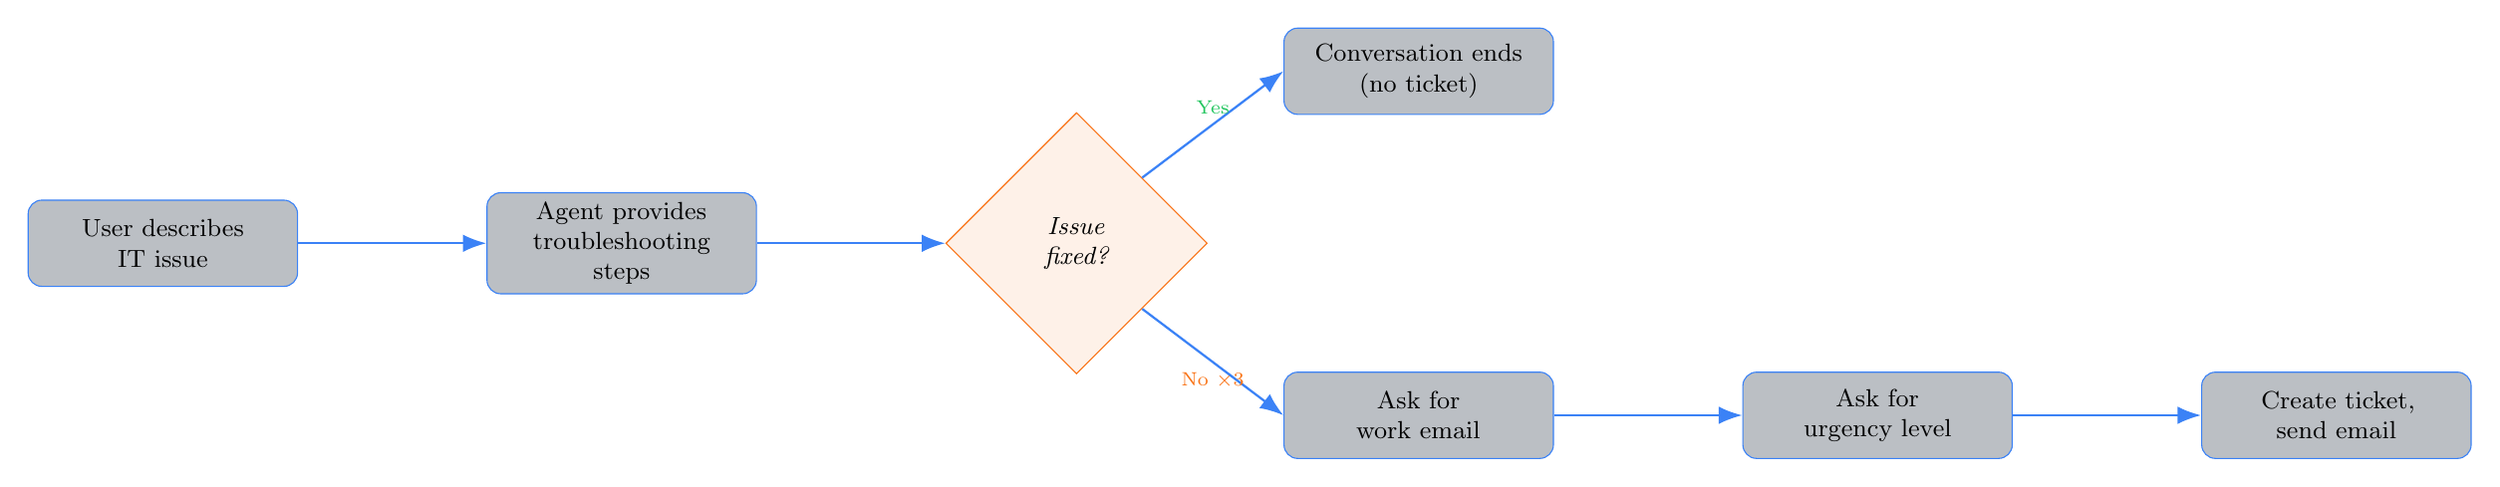
\begin{tikzpicture}[
  node distance=1.6cm and 2.4cm,
  box/.style={rectangle, rounded corners=5pt, draw=accent, fill=midbg!30,
               text width=3.2cm, align=center, minimum height=1.1cm, font=\small},
  decision/.style={diamond, draw=orange, fill=orange!10,
                   text width=2.2cm, align=center, font=\small\itshape},
  arrow/.style={-{Latex[length=3mm]}, thick, color=accent}
]

\node[box] (user)  {User describes\\ IT issue};
\node[box, right=of user] (help)  {Agent provides\\ troubleshooting\\ steps};
\node[decision, right=of help] (fixed) {Issue\\ fixed?};
\node[box, above right=0.8cm and 1.8cm of fixed] (resolved) {Conversation ends\\(no ticket)};
\node[box, below right=0.8cm and 1.8cm of fixed] (email)  {Ask for\\ work email};
\node[box, right=of email] (urgency) {Ask for\\ urgency level};
\node[box, right=of urgency] (ticket)  {Create ticket,\\ send email};

\draw[arrow] (user) -- (help);
\draw[arrow] (help) -- (fixed);
\draw[arrow] (fixed.north east) -- node[above, font=\scriptsize, color=green]{Yes} (resolved.west);
\draw[arrow] (fixed.south east) -- node[below, font=\scriptsize, color=orange]{No $\times$3} (email.west);
\draw[arrow] (email) -- (urgency);
\draw[arrow] (urgency) -- (ticket);

\end{tikzpicture}
\end{center}

%% ─────────────────────────────────────────────────────────────────────────────
\section{Original Production Architecture}
%% ─────────────────────────────────────────────────────────────────────────────

\begin{notebox}
  \textbf{Note:} This section describes the design pattern used in the production system.
  No internal system names, API endpoints, or proprietary configurations are disclosed.
  Internal identifiers have been anonymised.
\end{notebox}

\subsection{Microsoft Copilot Studio --- Dialog Engine}

Microsoft Copilot Studio (formerly Power Virtual Agents) hosted the conversational AI
agent. It was responsible for:

\begin{itemize}[leftmargin=*]
  \item \textbf{Topic management:} Separate dialog topics for each IT category
        (Hardware, Software, Network, Access), each with its own slot-filling flow.
  \item \textbf{Entity extraction:} Built-in entities for email addresses and custom
        entities for urgency level (High / Medium / Low) and system names (fuzzy-matched
        against the CMDB Configuration Item list).
  \item \textbf{Escalation logic:} If the agent's confidence score fell below 0.6 on
        intent classification, the conversation was handed off to a live agent queue.
  \item \textbf{Adaptive cards:} Quick-reply buttons for urgency selection were rendered
        as native Teams adaptive cards, providing a structured selection experience.
  \item \textbf{Trigger condition:} The agent was published as a Teams app and available
        in both personal chat and the IT Support shared channel.
\end{itemize}

\subsection{Power Automate --- Cloud Flow}

A cloud flow was triggered by an HTTP action from Copilot Studio when all required fields
were collected. The flow performed:

\begin{enumerate}[leftmargin=*, label=\arabic*.]
  \item \textbf{Input validation:} Email regex check, urgency enum validation, and
        required-field guard clauses.
  \item \textbf{Category classification:} A SharePoint lookup table mapped keywords in
        the issue description to one of five categories, determining the routing team.
  \item \textbf{Dataverse write:} A ``Create record'' action inserted the structured
        ticket into a custom Dataverse table with all pre-populated fields.
  \item \textbf{ITSM API call:} An HTTP action posted the ticket to the internal IT
        service management REST endpoint, which returned an incident number (INC-xxxxx).
  \item \textbf{Email notification:} The Office 365 Outlook connector sent an HTML
        confirmation email to the requestor, including the ticket ID, assigned team,
        and SLA commitment.
  \item \textbf{Return payload:} The flow returned the ticket ID and team assignment
        back to Copilot Studio, which displayed it to the user in Teams.
\end{enumerate}

\subsection{Data Layer --- Dataverse}

A custom Dataverse table stored every ticket record with the following schema:

\begin{center}
\begin{tabular}{lll}
\toprule
\textbf{Column} & \textbf{Type} & \textbf{Source} \\
\midrule
Description & Text (500) & Free-text from user \\
RequestorEmail & Email & Entity extracted by agent \\
Priority & Choice (H/M/L) & Urgency entity \\
AffectedSystem & Text & Optional slot \\
Category & Choice & SharePoint lookup \\
AssignedTeam & Choice & Derived from Category \\
IncidentNumber & Text & Returned by ITSM API \\
CreatedOn & Date/Time & System field (UTC) \\
Status & Choice & Default: Open \\
SLATarget & Date/Time & Calculated from Priority \\
\bottomrule
\end{tabular}
\end{center}

\subsection{ITSM Integration}

The internal IT service management system was integrated via its REST API using an HTTP
connector in Power Automate. Field mapping between Dataverse columns and ITSM schema
fields was defined in a mapping table within the flow, making it easy to update without
changing the Copilot Studio dialog.

Bi-directional synchronisation was implemented: when an agent closed a ticket in the ITSM
system, a second flow triggered on the status change and updated the corresponding Dataverse
record and sent the user a resolution notification via Teams.

\subsection{Microsoft Teams --- Deployment Channel}

The agent was published as a Teams app using the Copilot Studio ``Publish'' flow, which
generates a manifest and uploads it to the Teams admin centre for organisation-wide
deployment. Key channel features:

\begin{itemize}[leftmargin=*]
  \item Available in personal chat and the \emph{IT Support} shared channel.
  \item Adaptive cards rendered natively for quick-reply interactions.
  \item Proactive messages sent to the user when their ticket status changed.
\end{itemize}

\subsection{Data Flow --- Field Mapping Table}

\begin{center}
\begin{tabularx}{\linewidth}{X X X X}
\toprule
\textbf{User input} & \textbf{Agent entity} & \textbf{Dataverse field} & \textbf{ITSM field} \\
\midrule
Free-text description & issue\_description & Description & short\_description \\
Work email address & user\_email & RequestorEmail & caller\_id \\
High / Medium / Low & urgency\_level & Priority & priority (1/2/3) \\
Affected system (opt.) & affected\_system & AffectedSystem & cmdb\_ci \\
(derived) & category & Category & category \\
(derived) & assigned\_team & AssignedTeam & assignment\_group \\
(system) & --- & CreatedOn & opened\_at (UTC) \\
\bottomrule
\end{tabularx}
\end{center}

%% ─────────────────────────────────────────────────────────────────────────────
\section{Public Demo Architecture}
%% ─────────────────────────────────────────────────────────────────────────────

\subsection{Design Goals}

The demo was built to faithfully recreate the user experience and data flow of the
production system using only freely available, non-proprietary tooling. The three
design goals were:

\begin{enumerate}[leftmargin=*, label=\arabic*.]
  \item \textbf{Real AI, real storage, real email} — no mocked responses or fake data.
  \item \textbf{Privacy by design} --- PII stripped from messages before reaching any
        third-party AI provider.
  \item \textbf{Zero operational cost} --- deployable and runnable indefinitely on free
        service tiers.
\end{enumerate}

\subsection{Technology Stack}

\begin{center}
\begin{tabular}{lll}
\toprule
\textbf{Layer} & \textbf{Service} & \textbf{Replaces (production)} \\
\midrule
Conversational AI & Groq API (Llama 3.3 70B) & Microsoft Copilot Studio \\
Backend serverless & Vercel Functions (Node.js 18) & Power Automate Cloud Flow \\
Ticket storage & Supabase (PostgreSQL) & Microsoft Dataverse \\
Email delivery & Resend & Office 365 Outlook connector \\
Hosting & Vercel (static + functions) & SharePoint / Azure Static Web Apps \\
Frontend & Vanilla HTML / CSS / JS & Teams adaptive cards \\
\bottomrule
\end{tabular}
\end{center}

\subsection{Project File Structure}

\begin{lstlisting}[language=bash, caption={Repository layout}]
ryco-ai-support-agent-demo/
├── api/
│   ├── chat.js          # POST /api/chat  — AI handler, ticket creation
│   └── tickets.js       # GET  /api/tickets — live ticket table feed
├── css/
│   └── styles.css       # Full stylesheet + mobile responsive rules
├── data/
│   └── sample-tickets.json  # Static synthetic ticket dataset
├── js/
│   └── demo.js          # Frontend state machine & API client
├── supabase/
│   └── schema.sql       # tickets table DDL
├── index.html           # Landing / overview page
├── demo.html            # Interactive chat demo page
├── architecture.html    # Architecture diagram + component breakdown
├── package.json         # Node.js dependencies
├── vercel.json          # Deployment config (functions + CORS headers)
└── .gitignore           # .env, node_modules, .vercel excluded
\end{lstlisting}

%% ─────────────────────────────────────────────────────────────────────────────
\section{Backend Implementation}
%% ─────────────────────────────────────────────────────────────────────────────

\subsection{API Design}

The backend exposes two serverless functions on Vercel:

\begin{center}
\begin{tabular}{llll}
\toprule
\textbf{Route} & \textbf{Method} & \textbf{Input} & \textbf{Output} \\
\midrule
\texttt{/api/chat} & POST & \texttt{\{messages, sessionId, userEmail\}} & \texttt{\{message, phase, ticket\}} \\
\texttt{/api/tickets} & GET & --- & Array of last 20 ticket rows \\
\bottomrule
\end{tabular}
\end{center}

Both functions are written in CommonJS (required by Vercel's Node.js runtime) and exported
as \inlinecode{module.exports = async function handler(req, res)}.

\subsection{System Prompt Engineering}
\label{sec:systemprompt}

The AI's behaviour is entirely controlled by a structured system prompt that encodes the
two-phase conversation protocol. The prompt is divided into five sections:

\begin{enumerate}[leftmargin=*, label=\arabic*.]
  \item \textbf{PHASE 1 — TROUBLESHOOT:} Instructs the model to acknowledge the issue,
        provide 1--2 specific and tailored troubleshooting steps, ask the user to report
        back, and append \inlinecode{<PHASE>helping</PHASE>}. If the user reports success,
        the model ends with \inlinecode{<PHASE>resolved</PHASE>}. After three failed
        attempts (or an explicit escalation request), the model transitions to Phase 2.
  \item \textbf{PHASE 2 — ESCALATE:} Instructs the model to ask for a work email address
        (\inlinecode{<PHASE>asking\_email</PHASE>}), then urgency
        (\inlinecode{<PHASE>asking\_urgency</PHASE>}), and finally to emit the structured
        ticket JSON inside \inlinecode{<TICKET\_DATA>} tags
        (\inlinecode{<PHASE>creating\_ticket</PHASE>}).
  \item \textbf{RULES:} Response length capped at 80 words; no repeated suggestions;
        no email request before troubleshooting fails; exactly one \inlinecode{<PHASE>}
        tag per response.
  \item \textbf{PRIVACY:} The model is informed that email addresses are replaced with
        \texttt{[REDACTED\_EMAIL]} before reaching it, and instructed to use that
        placeholder in the ticket JSON.
  \item \textbf{CATEGORY / TEAM / SLA:} A routing table maps issue keywords to team and
        SLA target (e.g.\ VPN/connectivity $\to$ Network Operations $\to$ 30 minutes).
\end{enumerate}

\subsubsection{Ticket Data Format}

When the model is ready to create a ticket, it emits a structured JSON block:

\begin{lstlisting}[language=JavaScript, caption={Ticket data format emitted by the AI}]
<TICKET_DATA>
{
  "email": "[REDACTED_EMAIL]",
  "issue_summary": "one-line title of the problem",
  "details": "full description including what troubleshooting was attempted",
  "urgency": "High|Medium|Low",
  "category": "Network / VPN|Access / Permissions|Hardware|Software / M365|General"
}
</TICKET_DATA>
\end{lstlisting}

The server parses this block, strips it from the display message, and uses it to write
the ticket to Supabase. The real email address is substituted back in at this point
(see Section~\ref{sec:pii}).

\subsection{PII Redaction}
\label{sec:pii}

A key privacy requirement was that no raw email addresses or phone numbers should leave
the server and reach Groq's API. The redaction is applied server-side, after receiving
the messages array from the client:

\begin{lstlisting}[language=JavaScript, caption={PII redaction in api/chat.js}]
const EMAIL_RE = /[a-zA-Z0-9._%+\-]+@[a-zA-Z0-9.\-]+\.[a-zA-Z]{2,}/g;
const PHONE_RE = /(\+?[\d][\d\s\-().]{6,}[\d])/g;

function redactPII(messages) {
  return messages.map(msg => ({
    ...msg,
    content: msg.content
      .replace(EMAIL_RE, '[REDACTED_EMAIL]')
      .replace(PHONE_RE, m => /\d{5,}/.test(m) ? '[REDACTED_PHONE]' : m),
  }));
}
\end{lstlisting}

The real email address is separately captured client-side (Section~\ref{sec:emailcapture})
and sent as \inlinecode{userEmail} in the request body --- outside the \inlinecode{messages}
array that gets redacted. When the server builds the ticket record, it restores the real
address:

\begin{lstlisting}[language=JavaScript, caption={Real email restored at ticket creation time}]
const resolvedEmail = userEmail ?? parsed.email;
\end{lstlisting}

This means the AI model only ever sees \texttt{[REDACTED\_EMAIL]}, while the Supabase
record and the confirmation email receive the real address.

\subsection{Phase Tag Parsing}

After receiving the model's response, the server extracts the phase tag and the (optional)
ticket data block:

\begin{lstlisting}[language=JavaScript, caption={Phase and ticket block extraction}]
const phaseMatch  = rawText.match(/<PHASE>([\s\S]*?)<\/PHASE>/);
const phase       = phaseMatch ? phaseMatch[1].trim() : 'helping';

const ticketMatch = rawText.match(/<TICKET_DATA>([\s\S]*?)<\/TICKET_DATA>/);

const cleanMessage = rawText
  .replace(/<PHASE>[\s\S]*?<\/PHASE>/, '')
  .replace(/<TICKET_DATA>[\s\S]*?<\/TICKET_DATA>/, '')
  .trim();
\end{lstlisting}

The user-facing \inlinecode{message} field in the response always has both tags stripped,
so the user never sees the structured metadata.

\subsection{Ticket Routing and SLA}

Server-side routing maps the AI's category string to the correct team and SLA target,
ensuring the AI's free-form category output never results in an unmapped ticket:

\begin{lstlisting}[language=JavaScript, caption={Team and SLA routing table}]
const TEAM_MAP = {
  Network:  { team: 'Network Operations',  sla: '30 minutes' },
  Hardware: { team: 'Hardware Support',    sla: '2 hours'    },
  Software: { team: 'Software Support',    sla: '1 hour'     },
  Access:   { team: 'Identity & Access',   sla: '30 minutes' },
  General:  { team: 'IT Support',          sla: '2 hours'    },
};
\end{lstlisting}

The map key is matched using the first word of the category field (e.g.\ ``Network / VPN''
matches ``Network''), with ``General'' as the fallback.

\subsection{Supabase Integration}

Tickets are persisted to a Supabase (PostgreSQL) database using the
\inlinecode{@supabase/supabase-js} client. The client is initialised once at module load
time with the service-role key (bypasses Row Level Security, appropriate for a server-side
function):

\begin{lstlisting}[language=JavaScript, caption={Supabase client initialisation}]
const supabase = process.env.SUPABASE_URL
  ? createClient(process.env.SUPABASE_URL, process.env.SUPABASE_SERVICE_KEY)
  : null;

// Insert at ticket creation time:
const { error } = await supabase.from('tickets').insert(ticket);
if (error) console.error('Supabase insert error:', error.message);
\end{lstlisting}

The guard (\inlinecode{process.env.SUPABASE\_URL ? ... : null}) ensures the function
does not crash if the environment variable is absent (e.g.\ during local development
without a \inlinecode{.env} file).

\subsection{Transactional Email (Resend)}

Confirmation emails are sent via Resend using the \inlinecode{resend} Node.js SDK.
The email is an HTML template matching the visual style of the demo site:

\begin{lstlisting}[language=JavaScript, caption={Resend email dispatch}]
if (resend) {
  await resend.emails.send({
    from:    process.env.FROM_EMAIL ?? 'onboarding@resend.dev',
    to:      ticket.email,
    subject: `IT Support Ticket Created — ${ticket.ticket_id}`,
    html:    buildEmail(ticket),
  }).catch(err => console.error('Resend error:', err.message));
}
\end{lstlisting}

The email includes the ticket ID, issue summary, priority (colour-coded), assigned team,
SLA commitment, and a footer referencing the demo.

\subsection{Ticket ID Generation}

Each ticket receives a synthetic incident ID in the format \texttt{\#INC-XXXXX} (5 digits,
starting above 20000 to resemble a production system with existing history):

\begin{lstlisting}[language=JavaScript, caption={Ticket ID generator}]
function genTicketId() {
  return '#INC-' + (20000 + Math.floor(Math.random() * 9000));
}
\end{lstlisting}

%% ─────────────────────────────────────────────────────────────────────────────
\section{Database Design}
%% ─────────────────────────────────────────────────────────────────────────────

\subsection{Schema}

The \inlinecode{public.tickets} table in Supabase holds every ticket created through the
demo:

\begin{lstlisting}[language=SQL, caption={Supabase schema (supabase/schema.sql)}]
CREATE TABLE IF NOT EXISTS public.tickets (
  id               UUID        PRIMARY KEY DEFAULT gen_random_uuid(),
  ticket_id        TEXT        NOT NULL,
  created_at       TIMESTAMPTZ NOT NULL DEFAULT NOW(),
  requestor_email  TEXT,
  requestor_name   TEXT,
  issue_summary    TEXT,
  issue_detail     TEXT,
  category         TEXT,
  assigned_team    TEXT,
  priority         TEXT,
  sla              TEXT,
  description      TEXT,
  status           TEXT        DEFAULT 'Open',
  resolved         BOOLEAN     DEFAULT FALSE,
  resolution_time  TEXT
);

CREATE INDEX IF NOT EXISTS tickets_created_at_idx
  ON public.tickets (created_at DESC);
\end{lstlisting}

\subsection{Query Pattern}

The \inlinecode{/api/tickets} endpoint retrieves the most recent 20 tickets, ordered by
creation timestamp descending:

\begin{lstlisting}[language=JavaScript, caption={Ticket table query}]
const { data, error } = await supabase
  .from('tickets')
  .select(
    'ticket_id, created_at, requestor_name, category, ' +
    'priority, assigned_team, resolved, resolution_time'
  )
  .order('created_at', { ascending: false })
  .limit(20);
\end{lstlisting}

%% ─────────────────────────────────────────────────────────────────────────────
\section{Frontend Implementation}
%% ─────────────────────────────────────────────────────────────────────────────

\subsection{Page Structure}

The demo consists of three HTML pages, all sharing a single CSS file:

\begin{center}
\begin{tabular}{lll}
\toprule
\textbf{Page} & \textbf{File} & \textbf{Purpose} \\
\midrule
Overview & \texttt{index.html} & Problem/solution, metrics, tech stack, demo steps \\
Interactive Demo & \texttt{demo.html} & Chat interface, step tracker, ticket display \\
Architecture & \texttt{architecture.html} & SVG diagram, component breakdown, field map \\
\bottomrule
\end{tabular}
\end{center}

\subsection{Client-Side State}

The frontend maintains four state variables throughout a conversation session:

\begin{lstlisting}[language=JavaScript, caption={Client-side state variables (js/demo.js)}]
let messages      = [];    // Full conversation history [{role, content}]
let lastTicket    = null;  // Set once API returns a ticket; blocks further input
let isThinking    = false; // Prevents double-sends while awaiting API response
let capturedEmail = null;  // Real email, sent as userEmail; never in messages[]
\end{lstlisting}

\subsection{Conversation History}

The API is stateless --- it holds no session memory. On every user message, the complete
conversation history is sent to \inlinecode{/api/chat}:

\begin{lstlisting}[language=JavaScript, caption={Request to /api/chat with full history}]
const res = await fetch('/api/chat', {
  method:  'POST',
  headers: { 'Content-Type': 'application/json' },
  body: JSON.stringify({
    messages,
    sessionId: getSessionId(),
    userEmail: capturedEmail
  }),
});
\end{lstlisting}

The model receives the full \inlinecode{messages} array (redacted), so it always has
context of the entire conversation to avoid repeating troubleshooting suggestions.

\subsection{Email Address Capture}
\label{sec:emailcapture}

When the user types their email address, it is captured on the client \emph{before} the
message is added to the \inlinecode{messages} array. The regex match runs synchronously
on the raw input string:

\begin{lstlisting}[language=JavaScript, caption={Client-side email capture}]
if (!capturedEmail) {
  const emailMatch = text.match(
    /[a-zA-Z0-9._%+\-]+@[a-zA-Z0-9.\-]+\.[a-zA-Z]{2,}/
  );
  if (emailMatch) capturedEmail = emailMatch[0].toLowerCase();
}
\end{lstlisting}

\inlinecode{capturedEmail} is then sent separately as \inlinecode{userEmail} in the
request body. Inside the \inlinecode{messages} array, the same message will have its
email replaced by \texttt{[REDACTED\_EMAIL]} by the server's \inlinecode{redactPII()}
function before it reaches Groq.

\subsection{Phase-Driven UI}

The server returns a \inlinecode{phase} string with every response. The frontend uses
this to update the step tracker and decide whether to show urgency quick-reply buttons:

\begin{lstlisting}[language=JavaScript, caption={Phase map and step synchronisation}]
const PHASE_STEPS = {
  helping:         { done: [1, 2],             active: 3 },
  asking_email:    { done: [1, 2, 3, 4],       active: 5 },
  asking_urgency:  { done: [1, 2, 3, 4, 5],    active: 6 },
  creating_ticket: { done: [1, 2, 3, 4, 5, 6], active: 7 },
  resolved:        { done: [1, 2, 3],           active: null },
};

function syncSteps(phase, ticketDone) {
  for (let i = 1; i <= 8; i++) setStep(i, 'pending');
  if (ticketDone) {
    for (let i = 1; i <= 8; i++) setStep(i, 'done');
    return;
  }
  const map = PHASE_STEPS[phase] ?? PHASE_STEPS.helping;
  map.done.forEach(n => setStep(n, 'done'));
  if (map.active) setStep(map.active, 'active');
}
\end{lstlisting}

Quick-reply buttons for urgency selection are rendered only when
\inlinecode{phase === 'asking\_urgency'}:

\begin{lstlisting}[language=JavaScript, caption={Conditional quick-reply rendering}]
const opts = phase === 'asking_urgency'
  ? { quickReplies: [
      '[R] High  -- need it now',
      '[Y] Medium -- within the hour',
      '[G] Low   -- today is fine'
    ]}
  : {};

addMessage('bot', data.message, opts);
\end{lstlisting}

\subsection{Step Tracker}

The sidebar step tracker shows 8 labelled steps:

\begin{enumerate}[leftmargin=*, label=\arabic*., itemsep=2pt]
  \item Describe your IT issue
  \item Agent suggests a fix
  \item Try the troubleshooting steps
  \item Agent escalates to IT team
  \item Provide your work email
  \item Select urgency level
  \item Power Automate flow fires
  \item Ticket created \& confirmed
\end{enumerate}

Each step element carries one of three CSS classes: \inlinecode{pending},
\inlinecode{active}, or \inlinecode{done}, styled with distinct colours and
left-border indicators.

\subsection{Flow Animation}

When a ticket is created, a Power Automate--style flow animation runs in the sidebar,
revealing five sequential steps with a 560 ms delay between each:

\begin{lstlisting}[language=JavaScript, caption={Flow animation sequence}]
async function runFlowAnimation() {
  const badge = document.getElementById('flow-badge');
  badge.classList.remove('hidden');
  for (const id of ['fs1', 'fs2', 'fs3', 'fs4', 'fs5']) {
    await sleep(560);
    document.getElementById(id)?.classList.remove('hidden');
  }
}
\end{lstlisting}

The five displayed steps are:
\textit{Validating input fields\ldots} $\to$
\textit{Categorising ticket\ldots} $\to$
\textit{Creating record in ITSM\ldots} $\to$
\textit{Sending confirmation email\ldots} $\to$
\textit{\checkmark~Flow complete — 2.1s}.

\subsection{Ticket Card Display}

After the flow animation completes, the ticket card is populated from the API response
and scrolled into view. It displays all key fields: ticket ID, status, priority
(colour-coded), requestor, email, category, assigned team, SLA, creation timestamp,
and full description.

\subsection{Live Ticket Table}

A live ticket table at the bottom of the demo page queries \inlinecode{/api/tickets}
on page load and after each ticket creation. It displays the last 20 tickets from
Supabase, with columns: Ticket ID, Date, Requestor, Category, Priority, Assigned Team,
Resolved, and Resolution Time.

%% ─────────────────────────────────────────────────────────────────────────────
\section{Mobile Responsiveness}
%% ─────────────────────────────────────────────────────────────────────────────

Mobile support was added via CSS breakpoints at the bottom of \inlinecode{styles.css}:

\begin{center}
\begin{tabular}{llp{7cm}}
\toprule
\textbf{Breakpoint} & \textbf{Width} & \textbf{Changes applied} \\
\midrule
Tablet & $\leq$900px & Demo layout switches to single column; chat window
  gets \inlinecode{order:1}, sidebar \inlinecode{order:2} (chat above sidebar) \\
Mobile & $\leq$640px & Nav links at 12px; hero padding reduced; hero mockup
  hidden; Teams badge hidden; \inlinecode{\#chat-input font-size:16px}
  (prevents iOS Safari auto-zoom); \inlinecode{.chat-bubble max-width:82vw};
  \inlinecode{.chat-body max-height:55vh}; ticket fields stack to single column \\
\bottomrule
\end{tabular}
\end{center}

The CSS \inlinecode{order} property is used to reorder the chat window and sidebar on
mobile without changing the HTML DOM order, which preserves tab/accessibility order.

The \inlinecode{font-size: 16px} on the text input is a specific iOS Safari workaround:
the browser auto-zooms any input with a font size below 16px, which breaks the layout
on mobile.

%% ─────────────────────────────────────────────────────────────────────────────
\section{Privacy and Security}
%% ─────────────────────────────────────────────────────────────────────────────

\subsection{PII Handling Summary}

\begin{center}
\begin{tabular}{p{4.5cm}p{4cm}p{5cm}}
\toprule
\textbf{Data item} & \textbf{Where captured} & \textbf{Where it goes} \\
\midrule
User's email address & Client-side regex match on raw input & Sent as \texttt{userEmail} field (not in \texttt{messages}); restored at ticket creation; stored in Supabase; sent in confirmation email \\
Email in \texttt{messages} array & Any user turn & Replaced with \texttt{[REDACTED\_EMAIL]} by server before forwarding to Groq \\
Phone numbers & Any user turn & Replaced with \texttt{[REDACTED\_PHONE]} by server before forwarding to Groq \\
All other conversation text & \texttt{messages} array & Sent to Groq as-is \\
\bottomrule
\end{tabular}
\end{center}

\subsection{Secrets Management}

All API keys and database credentials are stored in:

\begin{itemize}[leftmargin=*]
  \item A local \inlinecode{.env} file (git-ignored via \inlinecode{.gitignore}).
  \item Vercel's encrypted environment variable store for production.
\end{itemize}

The \inlinecode{.gitignore} explicitly excludes:

\begin{lstlisting}[language=bash, caption={.gitignore entries}]
.env
.env.local
node_modules/
.vercel/
\end{lstlisting}

No keys are logged to the console or returned in API responses. The Supabase service-role
key is used only server-side and never exposed to the browser.

\subsection{CORS Policy}

CORS headers are configured in \inlinecode{vercel.json} to allow all origins for the
API routes (acceptable for a public demo; production would restrict to specific origins):

\begin{lstlisting}[language=JavaScript, caption={vercel.json CORS configuration}]
{
  "headers": [
    {
      "source": "/api/(.*)",
      "headers": [
        { "key": "Access-Control-Allow-Origin",  "value": "*" },
        { "key": "Access-Control-Allow-Methods", "value": "GET, POST, OPTIONS" },
        { "key": "Access-Control-Allow-Headers", "value": "Content-Type" }
      ]
    }
  ]
}
\end{lstlisting}

%% ─────────────────────────────────────────────────────────────────────────────
\section{Deployment}
%% ─────────────────────────────────────────────────────────────────────────────

\subsection{Vercel Configuration}

The project is deployed to Vercel as a hybrid static + serverless application. The
\inlinecode{vercel.json} configuration sets a 30-second maximum execution time for the
AI function (to accommodate Groq API latency under load):

\begin{lstlisting}[language=JavaScript, caption={vercel.json}]
{
  "version": 2,
  "functions": {
    "api/*.js": {
      "maxDuration": 30
    }
  }
}
\end{lstlisting}

No \inlinecode{runtime} key is specified --- Vercel auto-detects Node.js from
\inlinecode{package.json}'s \inlinecode{engines} field. Including
\inlinecode{"runtime": "nodejs18.x"} was found to cause a deploy failure
(``Function Runtimes must have a valid version''), as that format is specific to AWS
Lambda.

\subsection{Environment Variables (Production)}

The following environment variables must be set in the Vercel project dashboard:

\begin{center}
\begin{tabular}{ll}
\toprule
\textbf{Variable} & \textbf{Source} \\
\midrule
\texttt{GROQ\_API\_KEY} & Groq console → API Keys \\
\texttt{SUPABASE\_URL} & Supabase project → Settings → API → Project URL \\
\texttt{SUPABASE\_SERVICE\_KEY} & Supabase project → Settings → API → service\_role key \\
\texttt{RESEND\_API\_KEY} & Resend dashboard → API Keys \\
\texttt{FROM\_EMAIL} & \texttt{onboarding@resend.dev} (Resend sandbox sender) \\
\bottomrule
\end{tabular}
\end{center}

\subsection{Deployment Issues Encountered}

During the deployment process, several non-obvious issues were encountered and resolved:

\begin{description}[leftmargin=*, font=\bfseries]
  \item[npx cache corruption (ENOTEMPTY):] The \inlinecode{npx vercel} command failed
        with an \texttt{ENOTEMPTY} error caused by a corrupted npm cache directory.
        Resolved by running \inlinecode{npm cache clean --force} and installing Vercel
        globally (\inlinecode{npm install -g vercel}).

  \item[Invalid runtime key in vercel.json:] The initial \inlinecode{vercel.json}
        included \inlinecode{"runtime": "nodejs18.x"}, which is AWS Lambda notation.
        Vercel rejected it with ``Function Runtimes must have a valid version''.
        Fixed by removing the \inlinecode{runtime} key entirely.

  \item[Groq 401 Unauthorised:] The demo displayed ``AI service unavailable'' after
        deployment. Vercel logs showed a 401 from Groq. Root cause: the
        \inlinecode{GROQ\_API\_KEY} environment variable had been set as
        \texttt{gsk\_...gsk\_actualkey} (the placeholder from the \inlinecode{.env}
        template was inadvertently prepended to the real key). Fixed by correcting the
        key in both \inlinecode{.env} and the Vercel dashboard.

  \item[Supabase key with inline comment:] The \inlinecode{SUPABASE\_SERVICE\_KEY}
        was set with an inline comment:
        \texttt{sb\_secret\_... \# use the service\_role key}. The comment was
        included as part of the key value, causing authentication failures. Fixed by
        stripping the comment from both \inlinecode{.env} and the Vercel environment
        variable.

  \item[Vercel project name restriction:] The initial project name
        \texttt{ryco-ai-support-agent-demo} was rejected (three consecutive hyphens
        are not permitted). Deployed as \texttt{ryco-ai-support-demo} instead.
\end{description}

%% ─────────────────────────────────────────────────────────────────────────────
\section{Sample Ticket Data}
%% ─────────────────────────────────────────────────────────────────────────────

The file \inlinecode{data/sample-tickets.json} provides a static synthetic dataset
of 15 representative tickets. These are used for the architecture page and as a reference
for the live ticket table format. A representative subset is shown below:

\begin{center}
\begin{tabular}{llllll}
\toprule
\textbf{Ticket ID} & \textbf{Date} & \textbf{Category} & \textbf{Priority} & \textbf{Team} & \textbf{Resolved} \\
\midrule
\#INC-20481 & 2024-03-15 & Network / VPN & High & Network Ops & Yes (22 min) \\
\#INC-20479 & 2024-03-15 & Software / M365 & Medium & Software Support & Yes (1h 04m) \\
\#INC-20477 & 2024-03-14 & Hardware / Laptop & Low & Hardware Support & Yes (3h 20m) \\
\#INC-20474 & 2024-03-14 & Access / Permissions & High & Identity \& Access & Yes (18 min) \\
\#INC-20470 & 2024-03-13 & Software / Teams & Medium & Software Support & Yes (47 min) \\
\#INC-20468 & 2024-03-13 & Network / WiFi & High & Network Ops & Yes (31 min) \\
\#INC-20445 & 2024-03-10 & Software / M365 & High & Software Support & \textit{No — open} \\
\bottomrule
\end{tabular}
\end{center}

All names (James Smith, Priya Nair, Sara Okonkwo, etc.) and email addresses
(\texttt{j.smith@ryco.com}) are entirely synthetic. The domain \texttt{ryco.com} does
not correspond to any real organisation.

%% ─────────────────────────────────────────────────────────────────────────────
\section{Representative Impact}
%% ─────────────────────────────────────────────────────────────────────────────

\begin{notebox}
  The metrics below are \textbf{illustrative}, based on typical outcomes reported for
  similar IT support automation projects. They are not claimed as measured results from
  a specific deployment and are presented with that framing on the live site.
\end{notebox}

\begin{center}
\begin{tabular}{p{4cm}p{3cm}p{6cm}}
\toprule
\textbf{Metric} & \textbf{Value} & \textbf{Interpretation} \\
\midrule
Unstructured intake reduction & $\sim$80\% & Representative fraction of tickets that arrive with complete structured fields after agent deployment (vs.\ ad-hoc emails) \\
Repetitive ticket types automated & High volume & Common categories (VPN, password, M365 sync) that follow a predictable resolution path \\
First-response time improvement & Hours $\to$ Minutes & Typical improvement for automated ticket acknowledgement vs.\ manual triage \\
Additional staff required & 0 & No headcount added to handle the volume handled by the automation layer \\
\bottomrule
\end{tabular}
\end{center}

%% ─────────────────────────────────────────────────────────────────────────────
\section{Key Design Decisions}
%% ─────────────────────────────────────────────────────────────────────────────

\subsection{Stateless API with Client-Side History}

Rather than storing conversation state server-side (session tokens, Redis, etc.), the
full \inlinecode{messages} array is maintained in the browser and sent with every request.
This simplifies the backend significantly and is perfectly adequate for single-user demo
sessions. The tradeoff is increased request payload size, which is acceptable given that
conversations are short (typically under 10 turns).

\subsection{Tag-Based AI Output Protocol}

Using \inlinecode{<PHASE>} and \inlinecode{<TICKET\_DATA>} tags embedded in the model's
free-text output, rather than asking the model to return structured JSON at the top level,
was a deliberate choice. It allows the model to produce natural prose responses while
still exposing machine-readable metadata. The tags are reliably stripped before the user
sees the message.

\subsection{Two-Phase Conversation Design}

The decision to require the AI to attempt troubleshooting before escalating mirrors the
original production system's intent: many common issues can be self-resolved with the
right guidance, reducing unnecessary tickets. The 3-attempt limit prevents the experience
from becoming frustrating if the issue genuinely requires human intervention.

\subsection{PII Redaction Architecture}

Email addresses are captured client-side and sent out-of-band rather than being blocked
at the server level. This allows the real address to be used for the confirmation email
and Supabase record, while ensuring the LLM provider never receives it. The alternative
(masking at the server but never restoring) would have required a separate mechanism to
collect the email outside the chat flow entirely.

\subsection{Phase-Driven Step Tracker vs.\ Message Count}

An early implementation tracked progress by counting the number of messages exchanged.
This was replaced with the phase-tag approach because message count is unreliable (the
AI might take more or fewer turns to troubleshoot) whereas the phase tag is explicitly
emitted by the model at a semantically meaningful point in the conversation.

%% ─────────────────────────────────────────────────────────────────────────────
\section{Challenges and Lessons Learned}
%% ─────────────────────────────────────────────────────────────────────────────

\subsection{Prompt Engineering Stability}

Getting the model to reliably emit exactly one \inlinecode{<PHASE>} tag per response,
in the correct position, required several iterations of the system prompt. The key
insight was to give the model an explicit, rule-labelled section (``\textbf{RULES}'')
stating the tag requirement, rather than burying it in prose instructions. Structured
prompt sections with visual separators (\texttt{━━━}) improved compliance significantly.

\subsection{Environment Variable Formatting}

Inline comments in \inlinecode{.env} files (\texttt{KEY=value \# comment}) are not
stripped by all dotenv implementations. The comment became part of the key value,
causing authentication failures that were non-obvious to debug. The lesson: never
write inline comments in \inlinecode{.env} files; put explanatory text in a separate
\inlinecode{.env.example} file.

\subsection{Vercel vs.\ AWS Lambda Configuration}

Vercel's \inlinecode{vercel.json} has a different schema from AWS Lambda function
configuration. The \inlinecode{"runtime"} key is specific to Lambda and is rejected
by Vercel. Vercel auto-detects the runtime from \inlinecode{package.json}, so no
explicit runtime declaration is needed.

\subsection{iOS Safari Input Zoom}

iOS Safari auto-zooms any text input with a computed \inlinecode{font-size} below
\inlinecode{16px} when the input receives focus. This caused the chat layout to shift
jarringly on mobile. The fix is simple (\inlinecode{font-size: 16px} on the input
element) but easy to miss if you do not test on a real iOS device.

\subsection{Honest Metrics}

An early version of the landing page included specific performance figures. These were
revised to qualitative, representative language with an explicit disclaimer, for two
reasons: (1) the specific figures could not be publicly verified without disclosing
internal data, and (2) interviewers are more likely to trust honest framing than precise
numbers attached to a demo project.

%% ─────────────────────────────────────────────────────────────────────────────
\section{Conclusion}
%% ─────────────────────────────────────────────────────────────────────────────

This project demonstrates end-to-end ownership of an AI automation system --- from problem
framing and architecture design, through full-stack implementation, to production deployment
and observability. The demo faithfully reproduces the conversational UX and data flow of
a production enterprise system using freely available tooling, with no proprietary assets.

The core technical contributions are:

\begin{itemize}[leftmargin=*]
  \item A two-phase AI conversation protocol (troubleshoot-first, escalate-on-failure)
        encoded in a structured system prompt and enforced via phase tags.
  \item A privacy layer that redacts PII before any message leaves the server toward
        a third-party AI provider, while preserving the real data for legitimate use
        (ticket storage and email).
  \item A stateless serverless backend that integrates three external services (Groq,
        Supabase, Resend) within a single handler, with graceful fallback if any service
        is unconfigured.
  \item A phase-driven frontend state machine that synchronises UI progress, quick-reply
        options, and input locking with the AI's conversation state.
\end{itemize}

The live demo is accessible at:

\begin{center}
  \large\url{https://ryco-ai-support-demo.vercel.app}
\end{center}

%% ─────────────────────────────────────────────────────────────────────────────
\appendix
\section{Dependencies}
%% ─────────────────────────────────────────────────────────────────────────────

\begin{center}
\begin{tabular}{lll}
\toprule
\textbf{Package} & \textbf{Version} & \textbf{Purpose} \\
\midrule
\texttt{groq-sdk} & \textasciicircum0.15.0 & Groq API client (Llama 3.3 70B) \\
\texttt{@supabase/supabase-js} & \textasciicircum2.49.0 & Supabase PostgreSQL client \\
\texttt{resend} & \textasciicircum4.5.0 & Transactional email API client \\
\bottomrule
\end{tabular}
\end{center}

Runtime requirement: Node.js $\geq$ 18 (specified in \inlinecode{package.json} engines).

%% ─────────────────────────────────────────────────────────────────────────────
\section{Groq Model Selection}
%% ─────────────────────────────────────────────────────────────────────────────

The model used is \textbf{Llama 3.3 70B Versatile} (\texttt{llama-3.3-70b-versatile})
via Groq's inference API. This was selected because:

\begin{itemize}[leftmargin=*]
  \item Available on Groq's free tier with generous rate limits.
  \item Sufficient instruction-following capability to reliably emit structured tags.
  \item Fast inference (typically 1--3 seconds) due to Groq's LPU hardware.
  \item No data training on prompts under the free tier (per Groq's privacy policy
        at time of implementation).
\end{itemize}

Maximum token budget per response is set to 512 tokens, sufficient for an 80-word
prose response plus the structured JSON block.

%% ─────────────────────────────────────────────────────────────────────────────
\section{Full System Prompt}
%% ─────────────────────────────────────────────────────────────────────────────

\begin{lstlisting}[caption={Complete system prompt (api/chat.js)}]
You are an IT Support Agent for RYCO. You help employees resolve
IT issues through a two-phase approach: first try to fix it
yourself, then escalate if needed.

*** PHASE 1 - TROUBLESHOOT ***
When a user first describes an IT issue:
- Acknowledge it in one sentence
- Give 1-2 specific, actionable troubleshooting steps tailored
  to their exact problem
- Ask them to try and report back
- End your message with: <PHASE>helping</PHASE>

If the user says it WORKED -> congratulate them briefly, no
ticket needed. End with: <PHASE>resolved</PHASE>

If the user says it DIDN'T WORK -> try a different approach
(do NOT repeat the same suggestion).
End with: <PHASE>helping</PHASE>

After 3 failed troubleshooting attempts, OR if the user says
"just create a ticket" / "escalate" / "I give up":
- Acknowledge the issue persists, tell them you'll escalate
- Ask for their work email address
- End with: <PHASE>asking_email</PHASE>

*** PHASE 2 - ESCALATE ***
Once you have a valid email address:
- Confirm you have it
- Ask how urgent this is, listing three options on separate lines:
  High - need it resolved immediately
  Medium - within the next hour
  Low - today works
- End with: <PHASE>asking_urgency</PHASE>

Once the user selects urgency:
- Confirm you're creating the ticket
- End with <PHASE>creating_ticket</PHASE> then the ticket block

*** RULES ***
- Keep every response under 80 words
- Be specific with troubleshooting - tailor to what user said
- Never suggest the same fix twice
- Never ask for email before troubleshooting has failed
- Always end every response with exactly one <PHASE> tag
- <PHASE> and <TICKET_DATA> tags are stripped before user sees them

*** PRIVACY ***
Emails are replaced with [REDACTED_EMAIL] before reaching you.
Use [REDACTED_EMAIL] in ticket JSON - server restores real address.

*** CATEGORY / TEAM / SLA ***
Network / VPN -> VPN, WiFi, connectivity -> Network Operations -> 30 min
Access / Permissions -> password, MFA, locked out -> Identity & Access -> 30 min
Hardware -> laptop, monitor, keyboard, printer -> Hardware Support -> 2 hours
Software / M365 -> Outlook, Teams, Office, M365 -> Software Support -> 1 hour
Software -> app, crash, install, slow -> Software Support -> 1 hour
General -> anything else -> IT Support -> 2 hours

*** TICKET DATA FORMAT ***
<TICKET_DATA>
{
  "email": "[REDACTED_EMAIL]",
  "issue_summary": "one-line title",
  "details": "description including troubleshooting attempted",
  "urgency": "High|Medium|Low",
  "category": "Network / VPN|Access / Permissions|Hardware|
                Software / M365|Software|General"
}
</TICKET_DATA>
\end{lstlisting}

\end{document}
